%
% section 2.5
%
\setcounter{section}{4}
\section{Ασύρματα Δίκτυα}
Σε ένα ασύρματο δίκτυο, αντί για καλώδιο το μέσο διάδοσης είναι ο αέρας. Για τη μετάδοση χρησιμοποιούνται οπτικά σήματα, υπέρυθρες, ή (συνηθέστερα) ραδιοκύματα. 

\begin{figure}[!h]
  \centering
  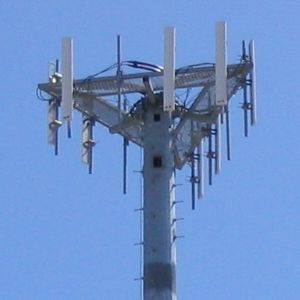
\includegraphics[width=0.55\textwidth]{images/chapter2/2-5}
  \caption {\textsl{Κεραία -- Σταθμός Εκπομπής Ασύρματου Σήματος}}
  \label{2-5}
\end{figure}

Τα ασύρματα δίκτυα με τη μεγαλύτερη εξάπλωση σήμερα είναι τα κυψελοειδή: πολλά από τα ασύρματα συστήματα αποτελούν εξειδίκευση ή γενίκευση των κυψελοειδών δικτύων. Κάθε δίκτυο καλύπτει μια περιοχή που ονομάζεται \emph{κυψέλη} χρησιμοποιώντας ένα \emph{σταθμό βάσης} και πολλούς ασύρματους \emph{χρήστες -- δέκτες}. 

Κάθε κυψέλη καλύπτει με σήμα μια περίπου εξαγωνική ή κυκλική περιοχή. Πολλές κυψέλες μαζί καλύπτουν ασύρματα μεγάλες εκτάσεις, όπως φαίνεται στο σχήμα \ref{2-6}.

\begin{figure}[!ht]
  \centering
  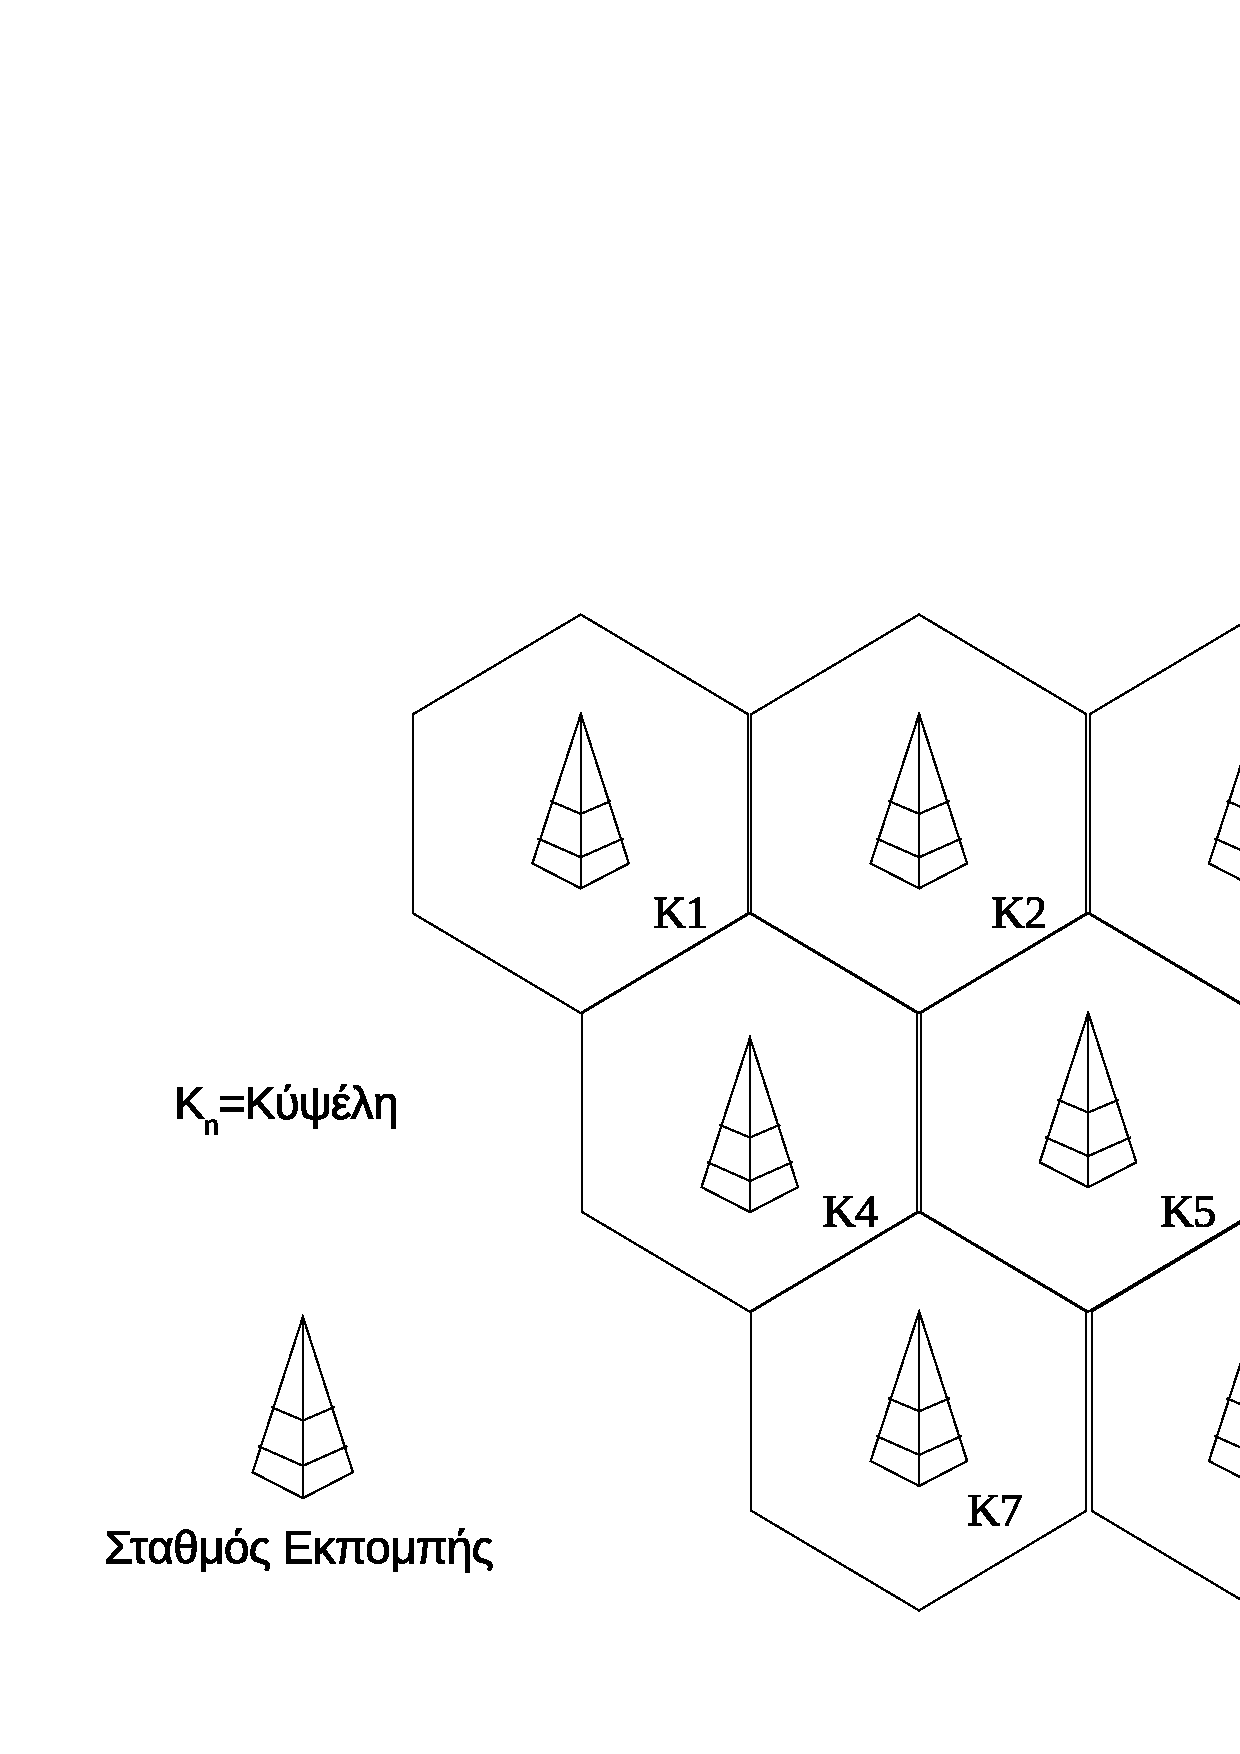
\includegraphics[width=0.90\textwidth]{images/chapter2/2-6}
  \caption {\textsl{Δίκτυο με Κυψέλες}}
  \label{2-6}
\end{figure}

Προϋπόθεση για τη σύνδεση των συσκευών μεταξύ τους είναι να έχουν εξοπλιστεί με κατάλληλο υλικό διεπαφής (π.χ. ασύρματες κάρτες δικτύου) που να επιτρέπει τη σύνδεση τους μέσω ασύρματης τεχνολογίας.

\begin{inthebox}
\textbf{Ένα καθημερινό παράδειγμα δικτύου με κυψέλες}

Ένα είδος ασύρματου δικτύου που χρησιμοποιεί κυψέλες είναι και το σύστημα κινητής τηλεφωνίας (GSM). Κάθε φορητή συσκευή (κινητό τηλέφωνο) είναι εφοδιασμένη με τον κατάλληλο πομποδέκτη και κυκλώματα που αφορούν τη ψηφιοποίηση των δεδομένων φωνής. Ο πάροχος της υπηρεσίας διαθέτει κυψέλες που γεωγραφικά καλύπτουν ολόκληρη τη χώρα. Καθώς το κινητό τηλέφωνο μετακινείται, συνδέεται κάθε φορά στην πιο κοντινή/ισχυρή κυψέλη χωρίς ο χρήστης να αντιλαμβάνεται τη μετάβαση από τη μια κυψέλη στην άλλη.\\
\end{inthebox}

Τα \textbf{ασύρματα τοπικά δίκτυα} ή WLAN (Wireless Local Area Network) επιτρέπουν σε ένα χρήστη κινητής συσκευής όπως ένας φορητός υπολογιστής, tablet ή smartphone να συνδέονται σε ένα τοπικό δίκτυο μέσω ασύρματης σύνδεσης ραδιοκυμάτων υψηλής συχνότητας.

\begin{figure}[!ht]
  \centering
  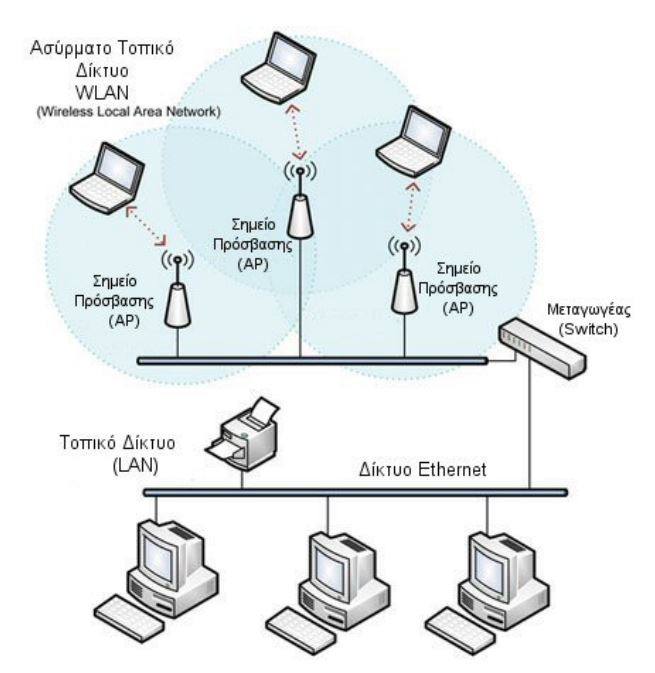
\includegraphics[width=0.65\textwidth]{images/chapter2/2-7}
  \caption {\textsl{Ασύρματο τοπικό δίκτυο συνδεόμενο με ενσύρματο δίκτυο}}
  \label{2-7}
\end{figure}

Στο σχήμα \ref{2-7} φαίνεται ένα τέτοιο δίκτυο που αποτελείται από τρία σημεία πρόσβασης (APs, Access Points) τα οποία σχηματίζουν ένα τοπικό ασύρματο δίκτυο και επιτρέπουν σε φορητές συσκευές που βρίσκονται στην εμβέλεια τους να συνδεθούν σε αυτά. Τα σημεία πρόσβασης συνδέονται μεταξύ τους και με το υπόλοιπο δίκτυο μέσω ενός μεταγωγέα (switch). Με αυτό το τρόπο δίνεται η δυνατότητα επέκτασης του τοπικού δικτύου και παροχής υπηρεσιών σε μεγαλύτερο αριθμό συσκευών. 